
\documentclass[11pt,compress,t,notes=noshow]{beamer}\usepackage[]{graphicx}\usepackage[]{color}

\makeatletter
\def\maxwidth{ %
  \ifdim\Gin@nat@width>\linewidth
    \linewidth
  \else
    \Gin@nat@width
  \fi
}
\makeatother

\definecolor{fgcolor}{rgb}{0.345, 0.345, 0.345}
\newcommand{\hlnum}[1]{\textcolor[rgb]{0.686,0.059,0.569}{#1}}%
\newcommand{\hlstr}[1]{\textcolor[rgb]{0.192,0.494,0.8}{#1}}%
\newcommand{\hlcom}[1]{\textcolor[rgb]{0.678,0.584,0.686}{\textit{#1}}}%
\newcommand{\hlopt}[1]{\textcolor[rgb]{0,0,0}{#1}}%
\newcommand{\hlstd}[1]{\textcolor[rgb]{0.345,0.345,0.345}{#1}}%
\newcommand{\hlkwa}[1]{\textcolor[rgb]{0.161,0.373,0.58}{\textbf{#1}}}%
\newcommand{\hlkwb}[1]{\textcolor[rgb]{0.69,0.353,0.396}{#1}}%
\newcommand{\hlkwc}[1]{\textcolor[rgb]{0.333,0.667,0.333}{#1}}%
\newcommand{\hlkwd}[1]{\textcolor[rgb]{0.737,0.353,0.396}{\textbf{#1}}}%
\let\hlipl\hlkwb

\usepackage{framed}
\makeatletter
\newenvironment{kframe}{%
 \def\at@end@of@kframe{}%
 \ifinner\ifhmode%
  \def\at@end@of@kframe{\end{minipage}}%
  \begin{minipage}{\columnwidth}%
 \fi\fi%
 \def\FrameCommand##1{\hskip\@totalleftmargin \hskip-\fboxsep
 \colorbox{shadecolor}{##1}\hskip-\fboxsep
     \hskip-\linewidth \hskip-\@totalleftmargin \hskip\columnwidth}%
 \MakeFramed {\advance\hsize-\width
   \@totalleftmargin\z@ \linewidth\hsize
   \@setminipage}}%
 {\par\unskip\endMakeFramed%
 \at@end@of@kframe}
\makeatother

\definecolor{shadecolor}{rgb}{.97, .97, .97}
\definecolor{messagecolor}{rgb}{0, 0, 0}
\definecolor{warningcolor}{rgb}{1, 0, 1}
\definecolor{errorcolor}{rgb}{1, 0, 0}
\definecolor{code}{rgb}{0.97, 0.96, 1.0}
\newenvironment{knitrout}{}{} % an empty environment to be redefined in TeX

\usepackage{alltt}
\usepackage[utf8]{inputenc}
\usepackage[ngerman]{babel}
\usepackage{dsfont}
\usepackage{verbatim}
\usepackage{amsmath}
\usepackage{amsfonts}
\usepackage{mathtools}
\usepackage{csquotes}
\usepackage{cmbright}
\usepackage{multirow}
\usepackage{longtable}
\usepackage{enumerate}
\usepackage[absolute,overlay]{textpos}
\usepackage{psfrag}
\usepackage{algorithm}
\usepackage{algpseudocode}
\usepackage{eqnarray}
\usepackage{bytefield}
\usepackage{animate}
\usepackage{tikz}
\usetikzlibrary{shapes,matrix,positioning,chains,arrows,shadows,decorations.pathmorphing,fit,backgrounds}
\usepackage{adjustbox}
\usepackage{colortbl}
\usepackage{tabularx} % for tables (incl. \hline)
\usepackage{arydshln} % Load after array, longtable, colortab and/or colortbl , otherwise problems with \hline in tabular env
\usepackage{etex} %increase registers for \dimenS to more than 256, otherwise we get "No room for a new \dimen"
\usepackage{graphicx}
\usepackage{booktabs} %used in epr lectures
\usepackage{bm} % bold greek letters
\usepackage{hyperref} % url citing
\usepackage{blkarray} % block arrays
\usepackage{listings} % block of code
\usepackage{xcolor} %colored math symbols
\usepackage{pgffor}
\usepackage{verbatimbox}
\usepackage{xcolor}

%some colors
\definecolor{checkgreen}{HTML}{18A126}
\definecolor{errorred}{HTML}{FF0000}
\definecolor{blockbg}{HTML}{F7F7F7}
\definecolor{gray}{HTML}{A0A0A0}

% basic latex stuff
\newcommand{\col}{\par\colorbox{code}{\parbox{\textwidth}{\theverbbox}}\par}
\newcommand{\eg}{e.\,g.\xspace} %for example
\newcommand{\ie}{i.\,e.\xspace} %that is to say...
\newcommand{\pkg}[1]{{\fontseries{b}\selectfont #1}} %fontstyle for R packages
\newcommand{\lz}{\vspace{0.5cm}} %vertical space
\newcommand{\oneliner}[1] % Oneliner for important statements
{\begin{block}{}\begin{center}\begin{Large}#1\end{Large}\end{center}\end{block}}
\def\SpAr{\quad \Rightarrow \quad}

%new environments
\newenvironment{vbframe}  %frame with breaks and verbatim
{
 \begin{frame}[containsverbatim,allowframebreaks]
}
{
\end{frame}
}

\newenvironment{vframe}  %frame with verbatim without breaks (to avoid numbering one slided frames)
{
 \begin{frame}[containsverbatim]
}
{
\end{frame}
}

\newenvironment{blocki}[1]   % itemize block
{
 \begin{block}{#1}\begin{itemize}
}
{
\end{itemize}\end{block}
}

\newenvironment{fragileframe}[2]{  %fragile frame with framebreaks
\begin{frame}[allowframebreaks, fragile, environment = fragileframe]
\frametitle{#1}
#2}
{\end{frame}}

\newcommand{\myframe}[2]{  %short for frame with framebreaks
\begin{frame}[allowframebreaks]
\frametitle{#1}
#2
\end{frame}}

\usepackage{../../style/lmu-lecture}

\let\code=\texttt
\let\proglang=\textsf

\setkeys{Gin}{width=0.9\textwidth}

\usepackage{tikz}
\usetikzlibrary{shapes,arrows,snakes, calc}

% Define block styles
\tikzstyle{decision} = [diamond, draw, text width=6em, text badly centered, node distance=4cm, inner sep=0pt]
\tikzstyle{decision2} = [diamond, draw, fill=customgreen!35, text width=6em, text badly centered, node distance=4cm, inner sep=0pt]

\tikzstyle{block} = [rectangle, draw, text width=14em, text centered, rounded corners, node distance=3cm, minimum height=4em]
\tikzstyle{line} = [draw, -latex']
\tikzstyle{cloud} = [draw, ellipse, node distance=3cm, minimum height=2em]

\title{Introduction to Deep Learning}
\author{Bernd Bischl}
\institute{Department of Statistics -- LMU Munich}
\date{WS 2021/2022}

\setbeamertemplate{frametitle}{\expandafter\uppercase\expandafter\insertframetitle}

\IfFileExists{upquote.sty}{\usepackage{upquote}}{}
\input{../../latex-math/basic-math}
\input{../../latex-math/basic-ml}
\input{../../latex-math/ml-nn}

\title{Deep Learning}
\date{}

\begin{document}
\newcommand{\titlefigure}{plots/AE_undercomplete.png}
%modify picture
\newcommand{\learninggoals}{
  \item Task and structure of an AE
  \item Undercomplete AEs
  \item Relation of AEs and PCA
}

\lecturechapter{Autoencoders - Basic Principle}
\lecture{I2DL}


\begin{vbframe}{Autoencoder-task and structure}

  \begin{itemize}
  \item Autoencoders (AEs) are %unsupervised approach for
  NNs for unsupervised learning of a lower dimensional feature representation from unlabeled training data.
  \item Task: Learn a compression of the data. 
  \item Autoencoders consist of two parts:
  \begin{itemize}
            \item \textbf{encoder} learns mapping from the data $\xv$ to a low-dimensional latent variable $\mathbf{z} = enc(\xv)$.
            \item \textbf{decoder} learns mapping back from latent $\mathbf{z} $ to a reconstruction  $\hat {\mathbf{x}} = dec(\mathbf{z})$ of $\xv$.
  \end{itemize}
    \item Loss function does not use any labels and measures the quality of the reconstruction compared to the input: 
    $$
      L\left(\xv, dec(enc(\xv))\right)
    $$
    \item Goal: Learn good \textbf{representation} $\mathbf{z}$ (also called \textbf{code}).
    %\item Autoencoding is a form of compression! Smaller latent space will force a larger training bottleneck

  \end{itemize}
  
%  \begin{itemize}
%    \item The basic idea of an autoencoder is to obtain a neural network, that is able to \textbf{reconstruct its input}.
%    \item[] $\Rightarrow$ Traditionally used for dimensionality reduction!
%    \item (Very) simple example: given the input vector (1, 0, 1, 0, 0), an autoencoder will try to output (1, 0, 1, 0, 0).
%    \item Therefore, we do not need class labels and pass over into the world of \textbf{unsupervised learning}.
%  \end{itemize}
\end{vbframe}
%%%%%%%%%%%%%%%%%%%%%%%%%%%%%%%%%%%%%%%%%%%%%%%%%%%%%%%%%%%%%%%%%%
%%%%%%%%%%%%%%%%%%%%%%%%%%%%%%%%%%%%%%%%%%%%%%%%%%%%%%%%%%%%%%%%%%
\begin{vbframe}{Autoencoder (AE)- computational graph}
%  \begin{itemize}
%    \item An autoencoder maps an input $x$ to an output $r$ (reconstruction)
%    \item We can distinguish its general architecture in the following manner:
%    \begin{itemize}
%      \item an encoder $z = enc(x)$ and
%      \item a decoder $r = dec(z)$ 
%    \end{itemize}
%    \item[] to generate the reconstruction.
%    \item We call $z$ the \textbf{internal representation} or \textbf{code}
%  \end{itemize}
%\framebreak
  The general structure of an AE as a computational graph:
  \begin{figure}
    \centering
    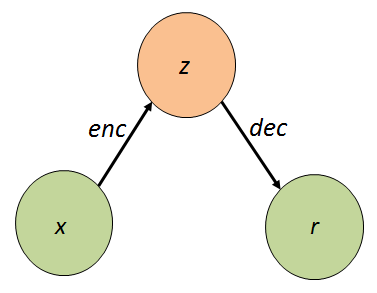
\includegraphics[width=5.5cm]{plots/autoencoder_basic_structure.png}
  \end{figure}
  \begin{itemize}
    \item An AE has two computational steps:
    \begin{itemize}
      \item the encoder $enc$, mapping $\xv$ to $\mathbf{z}$.
      \item the decoder $dec$, mapping $\mathbf{z}$ to $\hat\xv$.
    \end{itemize}
  \end{itemize}
\end{vbframe}
%%%%%%%%%%%%%%%%%%%%%%%%%%%%%%%%%%%%%%%%%%%%%%%%%%%%%%%%%%%%%%%%%%
%%%%%%%%%%%%%%%%%%%%%%%%%%%%%%%%%%%%%%%%%%%%%%%%%%%%%%%%%%%%%%%%%%
%\begin{frame}{Use case}
%
%Todo: Remove this slide?
%
%  \begin{itemize}
%    \item Practitioners utilize autoencoders, although they have access to labeled data.
%    \item[] $\Rightarrow$ Why?
%    \item Autoencoders may be used for:
%    \begin{itemize}
%      \item Learning a representation of the input data\\ $\Rightarrow$ dimensionality reduction \& pretraining
%      \item Advanced: some variants of the autoencoder can be regarded as generative models \\ $\Rightarrow$ may be used to draw synthetic data
%    \end{itemize}
%  \end{itemize}
%\end{frame}
%%%%%%%%%%%%%%%%%%%%%%%%%%%%%%%%%%%%%%%%%%%%%%%%%%%%%%%%%%%%%%%%%%
%%%%%%%%%%%%%%%%%%%%%%%%%%%%%%%%%%%%%%%%%%%%%%%%%%%%%%%%%%%%%%%%%%
% \frame{
% 
% \frametitle{Autoencoders - use case}
% 
%   \begin{itemize}
% 
%     \only<1-2>{\item Practitioners utilize autoencoders, although they have access to labeled data.}
%     \only<1-2>{\item[] $\Rightarrow$ Why?}
%     \only<2-2>{\item Autoencoders may be used for:}
%     \only<2>{\begin{itemize}
%       \only<2>{\item Learning a representation of the input data\\ $\Rightarrow$ dimensionality reduction \& pretraining}
%       \only<2>{\item Advanced: some variants of the autoencoder can be regarded as generative models \\ $\Rightarrow$ may be used to draw synthetic data}
%     \end{itemize}}
% 
%   \end{itemize}
% }
%%%%%%%%%%%%%%%%%%%%%%%%%%%%%%%%%%%%%%%%%%%%%%%%%%%%%%%%%%%%%%%%%%
%%%%%%%%%%%%%%%%%%%%%%%%%%%%%%%%%%%%%%%%%%%%%%%%%%%%%%%%%%%%%%%%%%

\section{Undercomplete Autoencoders}

\begin{frame}{Undercomplete Autoencoders}
  \only<1-2>{
    \begin{itemize}
      \item A naive implementation of an autoencoder would simply learn the identity $dec(enc(\xv)) = \mathbf{\hat x}$. 
      \item This would not be useful.
    \end{itemize}
  }
  \only<1>{
    \begin{figure}
    \centering
    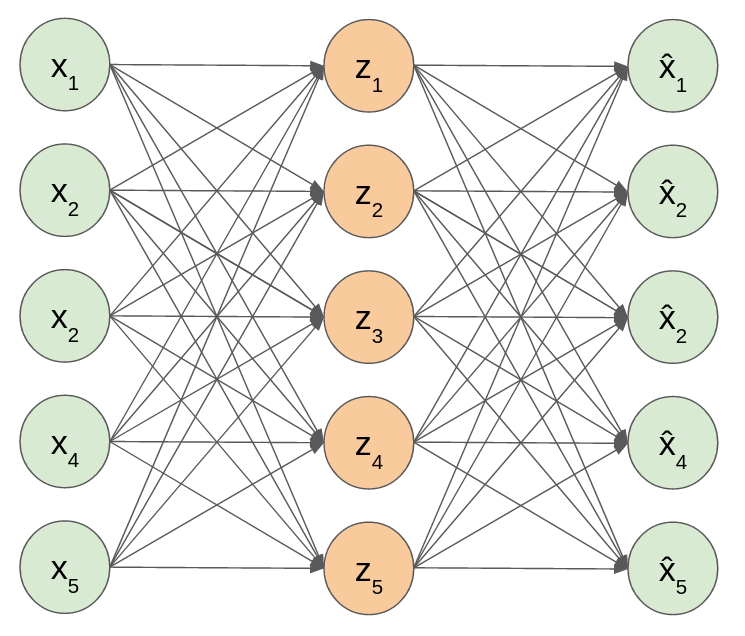
\includegraphics[width=0.6\textwidth]{plots/AE_naive1.png}
    \end{figure}
  }

  \only<2>{
    \begin{figure}
    \centering
    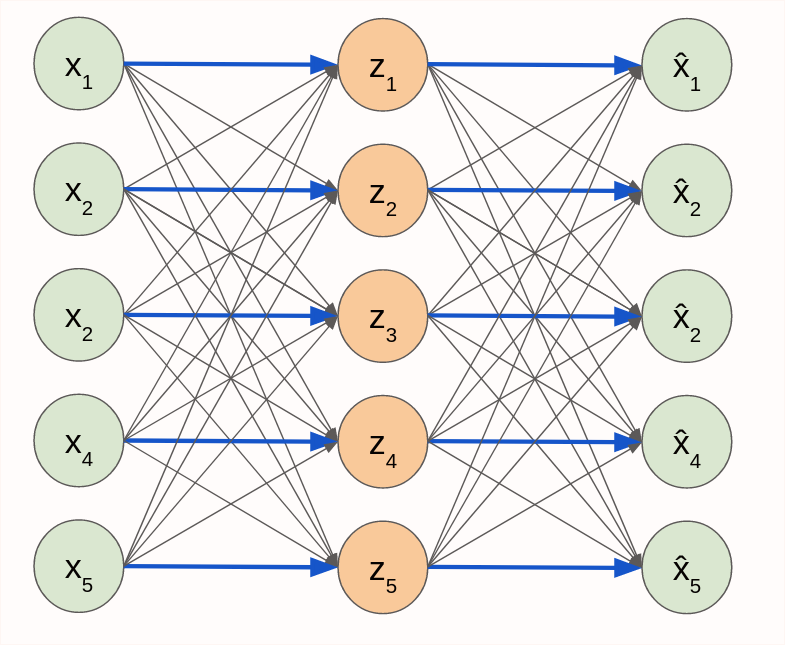
\includegraphics[width=0.6\textwidth]{plots/AE_naive2.png}
    \end{figure}
  }
  \only<3>{
    \begin{itemize}
      \item Therefore we have a \enquote{bottleneck} layer: We restrict the architecture, such that 
        $$
          \text{dim}(\mathbf{z}) < \text{dim}(\xv)
        $$
      \item Such an AE is called \textbf{undercomplete}. 
    \end{itemize}
  }  
  \only<4>{
    \begin{itemize}
      \item  In an undercomplete AE, the hidden layer has fewer neurons than the input layer. 
      \item[$\rightarrow$] That will force the AE to 
      \begin{itemize}
        \item  capture only the most salient features of the training data!
        \item  learn a \enquote{compressed} representation of the input.
      \end{itemize}   
    \end{itemize}
  }  

  \only<3-4>{
  %\vspace*{-0.3cm}
    \begin{figure}
    \centering
%<<<<<<< HEAD
    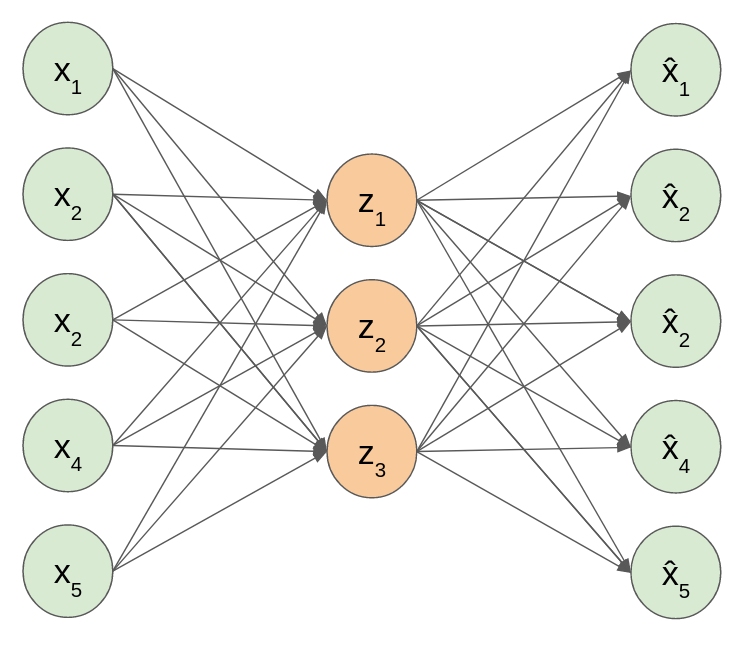
\includegraphics[width=0.55\textwidth]{plots/AE_undercomplete.png}
%=======
    %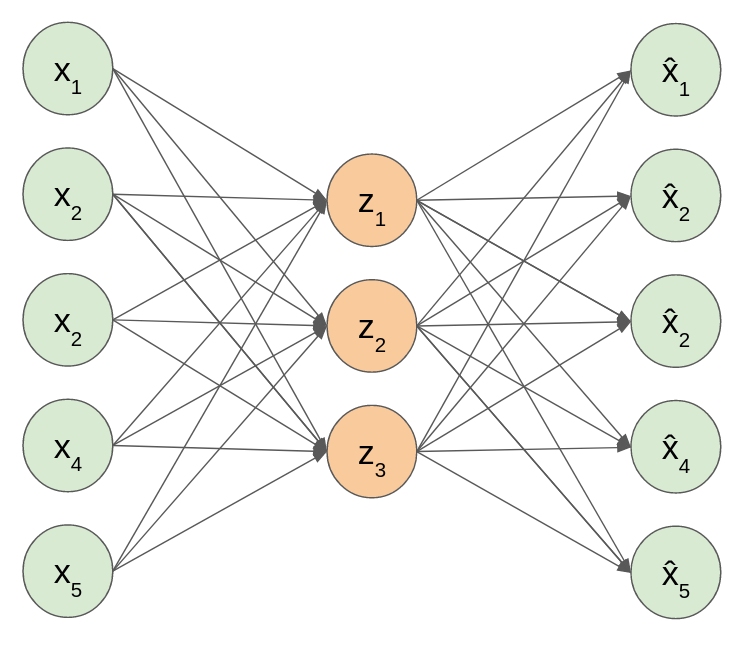
\includegraphics[width=0.55\textwidth]{plots/AE_undercomplete.png}
%>>>>>>> c67183e44e1e038de6a0abcc61f6f4ff2056b488
    \end{figure}
  }

    % $\to$ That will force the autoencoder to capture only the most salient features of the training data! 
    % \item If an AE simply learns the identity $dec(enc(\xv)) = \xv$, it would be of no use. In fact, we want the AE to learn a representation $\mathbf{z}$ that encodes \enquote{useful} or \enquote{significant} properties of the data.
    % \item Consequently, the autoencoder tries to learn a \enquote{compressed} representation of the input. 
    % \item %To extract such \enquote{useful} or \enquote{significant} properties, we introduce the \textbf{undercomplete autoencoder}.
    % One possibility to do so is to 
    % %\item Therefore, we 
    % restrict the architecture, such that \\ %$$dim(z) < dim(x)$$ 
    %  \textbf{code dimension $<$ input dimension}.
 %   \item Consequently, the undercomplete autoencoder tries to learn a \enquote{compressed} representation of the input.
  
\end{frame}

\begin{vbframe}{Undercomplete Autoencoders}

  \begin{itemize}
  %  \item In other words: In an undercomplete AE, the hidden layer has fewer neurons than the input layer.
  %   \item[] $\Rightarrow$ That will force the AE to 
  % \begin{itemize}
  % \item  capture only the most salient features of the training data!
  % \item  learn a \enquote{compressed} representation of the input.
  % \end{itemize}    
    \item %Learning such a net is 
    Training an AE is done by minimizing the risk with a loss function penalizing the reconstruction  $dec(enc(\xv))$ for differing from $\xv$. 
    \item The L2-loss 
    $$
    \|\xv - dec(enc(\xv))\|^2_2
    $$
    is a typical choice, but other loss functions are possible. 
%    \begin{itemize}
%      \item Typical choice: MSE
%    \end{itemize}
%    \item[]
    \item For optimization, the same optimization techniques as for standard feed-forward nets are applied (SGD, RMSProp, ADAM,...).
    \item[]
 %   \item How could a potential architecture of an undercomplete autoencoder look like for our (very) simple example?
  %  \item[] Reminder: $x = (1, 0, 1, 0, 0)$
  \end{itemize}

\end{vbframe}


\begin{frame}{Experiment: Learn to encode MNIST}
  \begin{itemize}
    \item Let us try to compress the MNIST data as good as possible.
    \item We train undercomplete AEs % to learn the best possible representation 
    %\item We fit the autoencode
     with different dimensions of the internal representation $\mathbf{z}$ (.i.e. different \enquote{bottleneck} sizes).
  \end{itemize}
  \begin{figure}
    \centering
    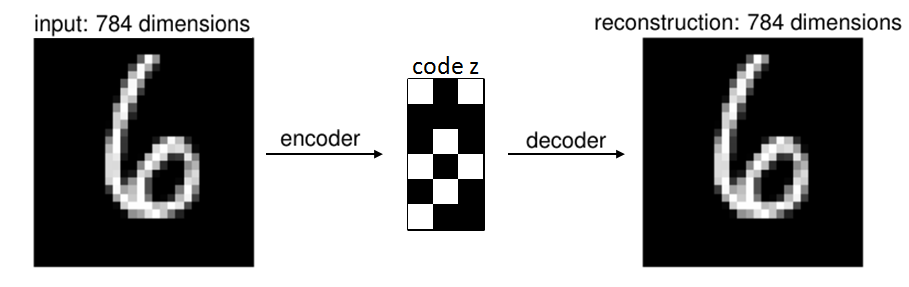
\includegraphics[width=11cm]{plots/autoencoder_mnist_problem.png}
    \caption{Flow chart of our our autoencoder: reconstruct the input with fixed dimensions $dim(\mathbf{z}) \leq dim(\xv)$.}
  \end{figure}
\end{frame}
%%%%%%%%%%%%%%%%%%%%%%%%%%%%%%%%%%%%%%%%%%%%%%%%%%%%%%%%%%%%%%%%%%
%%%%%%%%%%%%%%%%%%%%%%%%%%%%%%%%%%%%%%%%%%%%%%%%%%%%%%%%%%%%%%%%%%
\begin{frame}{Experiment: Learn to encode MNIST}
  \begin{figure}
    \centering
    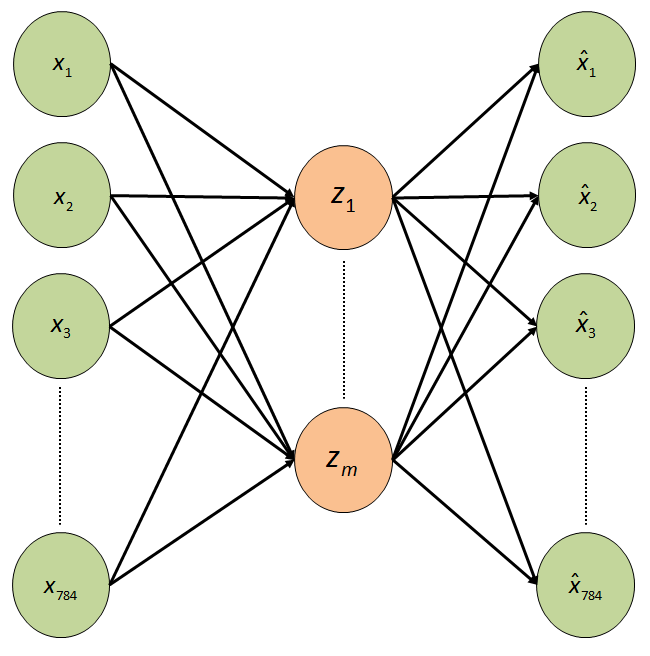
\includegraphics[width=6.5cm]{plots/autoencoder_mnist_example.png}
    \caption{Architecture of the autoencoder.}
  \end{figure}
\end{frame}

%%%%%%%%%%%%%%%%%%%%%%%%%%%%%%%%%%%%%%%%%%%%%%%%%%%%%%%%%%%%%%%%%%
%%%%%%%%%%%%%%%%%%%%%%%%%%%%%%%%%%%%%%%%%%%%%%%%%%%%%%%%%%%%%%%%%%
\frame{

\frametitle{Experiment: Learn to encode MNIST}
%%%%
%%%%%
%%%%%%%%
%%%%%%%%%%%
  \center
  \begin{figure}
  
    \only<1>{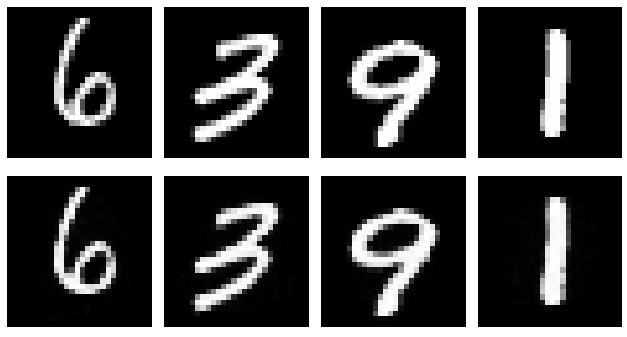
\includegraphics[width=11.2cm]{plots/784.png}}%
    \only<2>{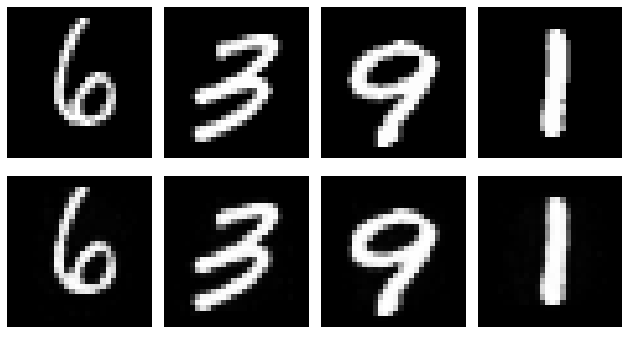
\includegraphics[width=11.2cm]{plots/256.png}}%
    \only<3>{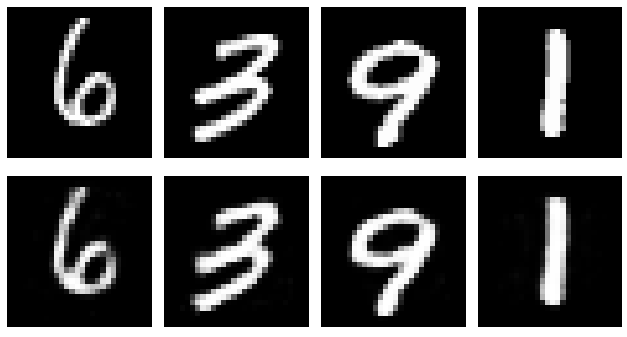
\includegraphics[width=11.2cm]{plots/64.png}}%
    \only<4>{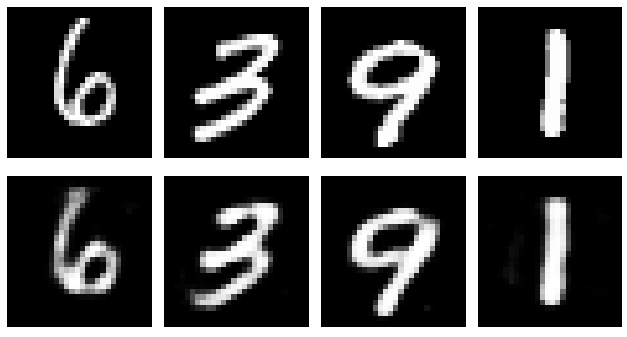
\includegraphics[width=11.2cm]{plots/32.png}}%
    \only<5>{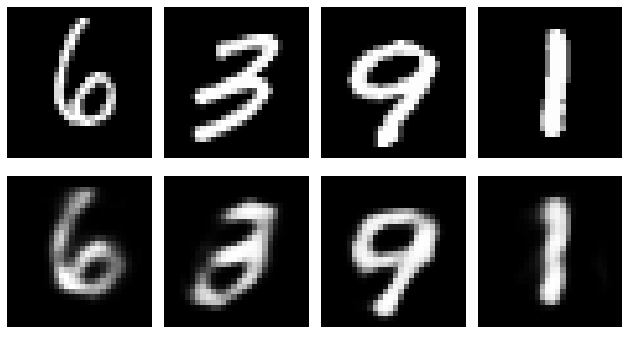
\includegraphics[width=11.2cm]{plots/16.png}}%
    \only<6>{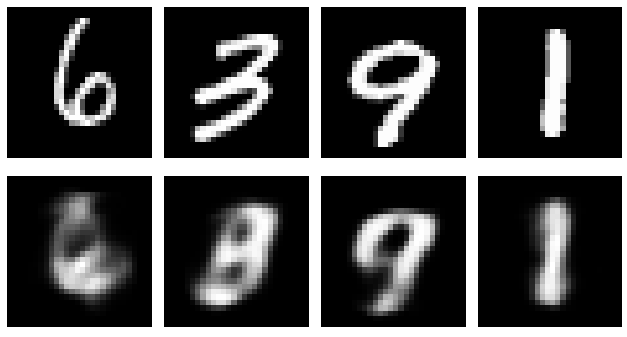
\includegraphics[width=11.2cm]{plots/8.png}}%
    \only<7>{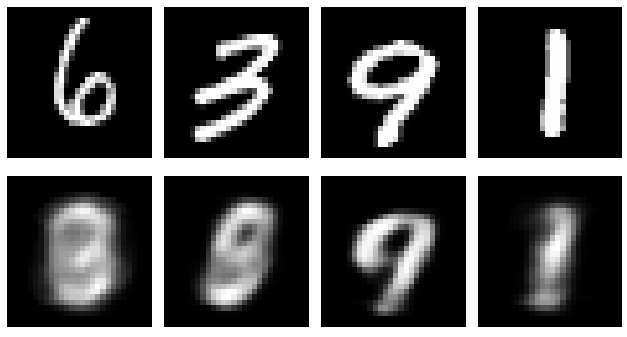
\includegraphics[width=11.2cm]{plots/4.png}}%
    \only<8>{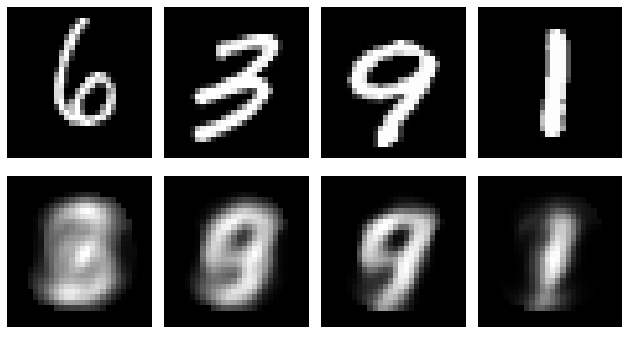
\includegraphics[width=11.2cm]{plots/2.png}}%
    \only<9>{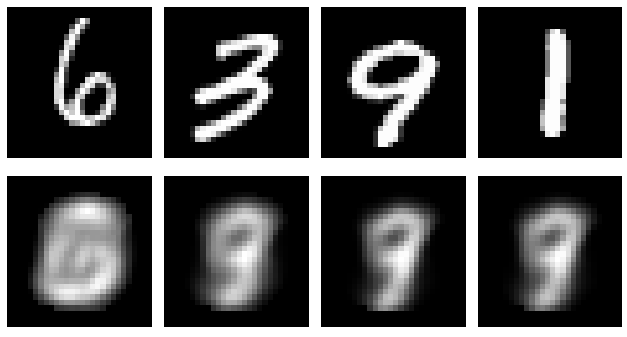
\includegraphics[width=11.2cm]{plots/1.png}}%
    \caption{The top row shows the original digits, the bottom row the reconstructed ones.}
    
  \end{figure}
  
  \vspace{-0.3cm}
  
  \begin{itemize}
  
    \only<1>{\item $dim(\mathbf{z}) = 784 = dim(\xv)$.}
    \only<2>{\item $dim(\mathbf{z}) = 256$.}
    \only<3>{\item $dim(\mathbf{z}) = 64$.}
    \only<4>{\item $dim(\mathbf{z}) = 32$.}
    \only<5>{\item $dim(\mathbf{z}) = 16$.}
    \only<6>{\item $dim(\mathbf{z}) = 8$.}
    \only<7>{\item $dim(\mathbf{z}) = 4$.}
    \only<8>{\item $dim(\mathbf{z}) = 2$.}
    \only<9>{\item $dim(\mathbf{z}) = 1$.}
    
  \end{itemize}
  
}

\begin{vbframe}{Increasing the Capactiy of AEs}

Increasing the number of layers adds capacity to autoencoders: 


  \begin{figure}
  \centering
  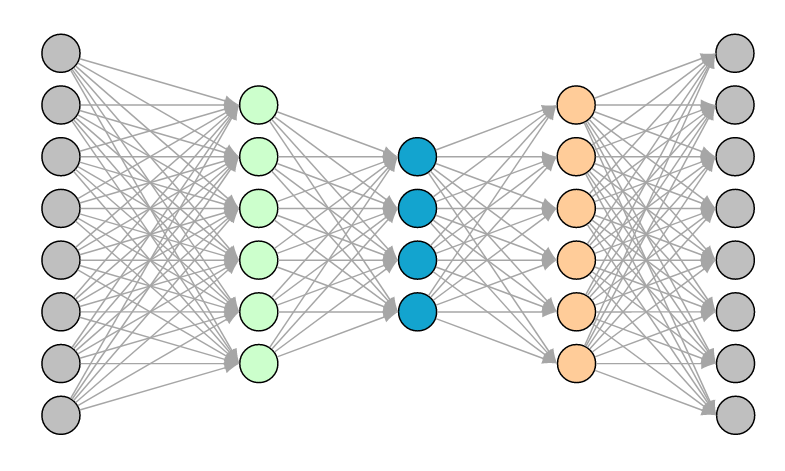
\includegraphics[width=0.9\textwidth]{plots/AE_increased_capacity.png}
  \end{figure}


\end{vbframe}

\section{Autoencoders as Principal Component Analysis}

\begin{vbframe}{AEs as Principal Component Analysis}

  \begin{itemize}
    \item Consider a undercomplete autoencoder with
    \begin{itemize}
      \item \textbf{linear} encoder function $enc(\xv)$, and
      \item \textbf{linear} decoder function $dec(\pmb{z})$.
    \end{itemize}  
    \item The L2-loss $\|\xv-dec(enc(\xv))\|^2_2$ is employed and inputs are normalized to zero mean.   
    \item %In other words: 
    We want to find the \textbf{linear projection} of the data with the minimal L2-reconstruction error.

    \begin{figure}
      \centering
      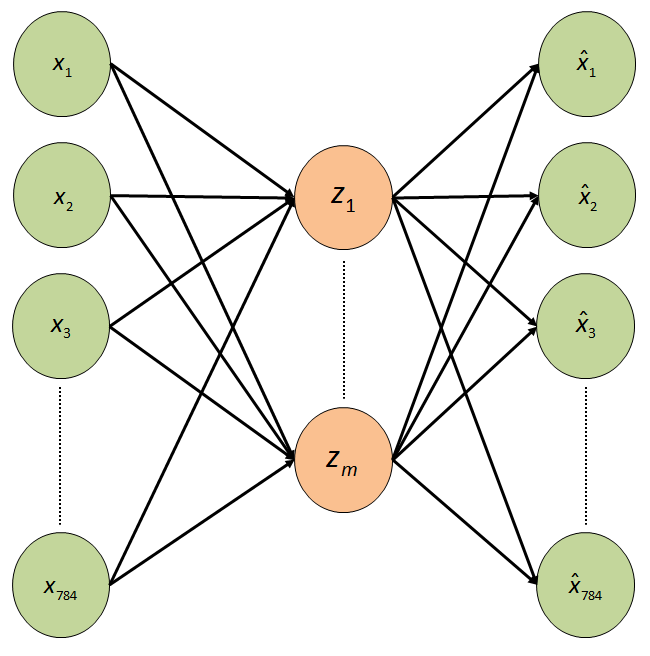
\includegraphics[width=0.3\textwidth]{plots/autoencoder_mnist_example.png}
    \end{figure}

    \framebreak 

    \item It can be shown that %, given a $\text{dim}(\bm{z}) = k$, 
    the optimal solution is an \textbf{orthogonal} linear transformation (i.e. a rotation of the coordinate system) given by the $\text{dim}(\bm{z}) = k$ singular vectors with largest singular values. 

    \begin{figure}
    \centering
    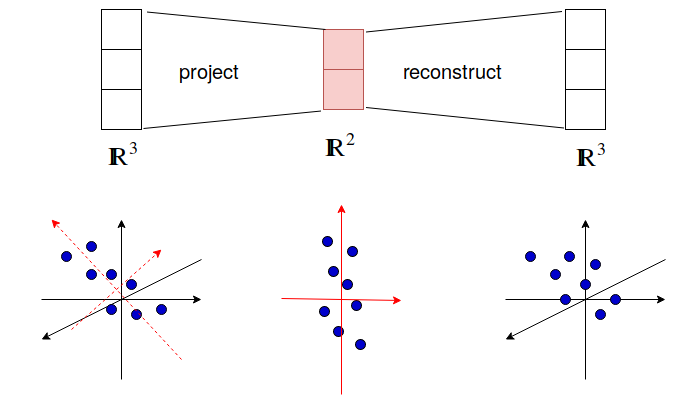
\includegraphics[width=0.7\textwidth]{plots/PCA_AE.png}
    \end{figure}

    \framebreak 

    \item This is an equivalent formulation to \textbf{Principal Component Analysis (PCA)}, which uses an orthogonal transformation to convert a set of observations of possibly correlated variables into a set of values of linearly uncorrelated variables called \textbf{principal components}. 
    \item The transformation is defined in such a way that the first principal component has the largest possible variance (i.e., accounts for as much of the variability in the data as possible).  
    \begin{figure}
    \centering
    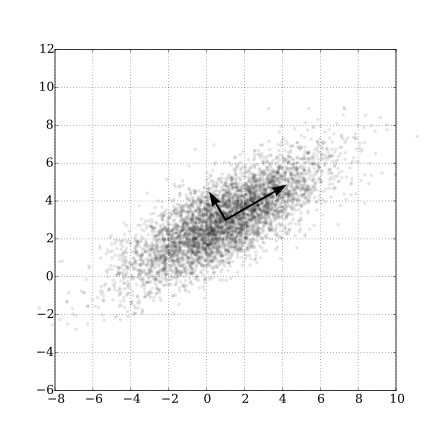
\includegraphics[width=3.5cm]{plots/PCA.png}
    \end{figure}

    \framebreak 

    \item The formulations are equivalent: \enquote{Find a linear projection into a $k$-dimensional space that ...}
    \begin{itemize}
      \item \enquote{... minimizes the L2-reconstruction error} (AE-based formulation).
      \item \enquote{... maximizes the variance of the projected datapoints} (statistical formulation). 
    \end{itemize}
  
   % \framebreak 

    \item An AE with a non-linear decoder/encoder can be seen as a non-linear generalization of PCA.

    \vspace*{-0.2cm}

    \begin{figure}
    \begin{center}
    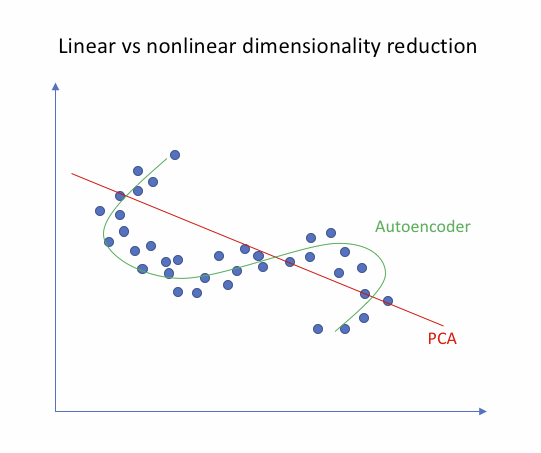
\includegraphics[width=0.3\textwidth]{plots/manifold1.png}
    \caption{Credits: Jeremy Jordan \enquote{Introduction to autoencoders}}
    \end{center}
    \end{figure}

  \end{itemize}
  
\end{vbframe}


%%%%%%%%%%%%%%%%%%%%%%%%%%%%%%%%%%%%%%%%%%%%%%%%%%%%%%%%%%%%%%%%%%
%%%%%%%%%%%%%%%%%%%%%%%%%%%%%%%%%%%%%%%%%%%%%%%%%%%%%%%%%%%%%%%%%%

\begin{vbframe}
\frametitle{References}
\footnotesize{
\begin{thebibliography}{99}
%%%%%%%%%%%%%%%%%%%%%%%%%%%%%%%%%%
\bibitem[Ian Goodfellow et al., 2016]{1} Ian Goodfellow, Yoshua Bengio and Aaron Courville (2016)
\newblock Deep Learning
\newblock \emph{\url{http://www.deeplearningbook.org/}}
%%%%%%%%%%%%%%%%%%%%%%%%%%%%%%%%%%

\end{thebibliography}
}
\end{vbframe}


\endlecture
\end{document}